% UTF-8
% pt-BR
\def\mypath{mathematics/2}

\newcommand\inlinebox[2][-0.5]{\raisebox{#1\height}{#2}}

\begin{question}
	\newcommand\mycoloneqq{\ensuremath{\mathrel{\mathop:}=}} % Thanks to The Comprehensive LaTeX Symbol List, p.48, 2015.

	Considere os vetores geométricos $\vec u$ e $\vec v$ ilustrados abaixo.
	Desenhe o vetores
	\begin{inlineenum}
		\inlineitem $\vec u + \vec v$,
		\inlineitem $\vec u - \vec v$ e
		\inlineitem $\frac{3}{2}\vec u$
	\end{inlineenum}

	\begin{center}
		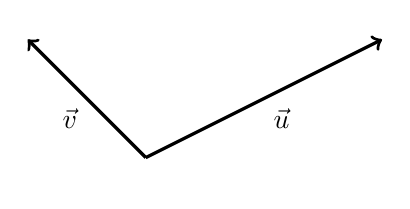
\begin{tikzpicture}[scale=1.5]
	\clip (-1,-0.2) rectangle (2,1.1);

	% \vec u
	\draw[very thick] [->] (0,0) -- (2,1);
	\draw (1,0.5) node[anchor=north west] {$\vec u$};

	% \vec v
	\draw[very thick] [->] (0,0) -- (-1,1);
	\draw (-0.5,0.5) node[anchor=north east] {$\vec v$};

\end{tikzpicture}
	\end{center}

	\begin{answer}
		\begin{enumerate}
			\item \inlinebox{\input{\mypath/figures/u_v_item_a_head_to_tail}} ou \inlinebox{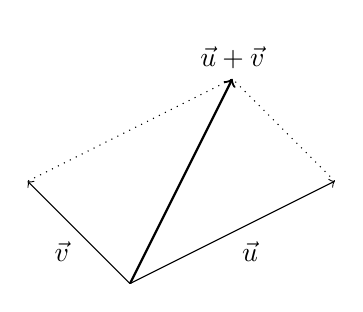
\begin{tikzpicture}[scale=1.3]
	\clip (-1,0) rectangle (2,2.5);

	% \vec u
	\draw[thin] [->] (0,0) -- (2,1);
	\draw (1,0.5) node[anchor=north west] {$\vec u$};

	% \vec v
	\draw[thin] [->] (0,0) -- (-1,1);
	\draw (-0.5,0.5) node[anchor=north east] {$\vec v$};

	% \vec u + \vec v
	\draw[thick] [->] (0,0) -- (1,2);
	\draw (1,2) node[anchor=south] {$\vec u + \vec v$};

	% Help lines
	\draw[dotted] [-] (2,1) -- (1,2) -- (-1,1);

\end{tikzpicture}}

			\item \inlinebox{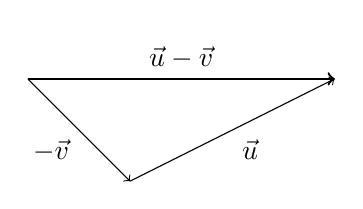
\begin{tikzpicture}[scale=1.3]
	\clip (-1,0) rectangle (2,1.5);

	% \vec u
	\draw[thin] [->] (0,0) -- (2,1);
	\draw (1,0.5) node[anchor=north west] {$\vec u$};

	% \vec -v
	\draw[thin] [<-] (0,0) -- (-1,1);
	\draw (-0.5,0.5) node[anchor=north east] {$-\vec v$};

	% \vec u + \vec v
	\draw[thick] [->] (-1,1) -- (2,1);
	\draw (0.5,1) node[anchor=south] {$\vec u - \vec v$};

\end{tikzpicture}}

			\item \inlinebox{\begin{tikzpicture}[scale=1.3]
	\clip (-1,0) rectangle (3,2);

	% 3/2 \vec u
	\draw[thick] [->] (0,0) -- (3,3/2);
	\draw (9/4,9/8) node[anchor=north west] {$\frac{3}{2}\vec u$};

	% \vec u
	\draw[thin] [->] (0,0) -- (2,1);
	\draw (1,0.5) node[anchor=north west] {$\vec u$};

	% \vec v
	\draw[thin] [->] (0,0) -- (-1,1);
	\draw (-0.5,0.5) node[anchor=north east] {$\vec v$};

\end{tikzpicture}}
		\end{enumerate}
	\end{answer}

	\begin{solution}
		\begin{enumerate}
			\item
			Pela definição, \inlinebox{\input{\mypath/figures/u_v_item_a_head_to_tail}}, ou pela regra do paralelogramo: \inlinebox{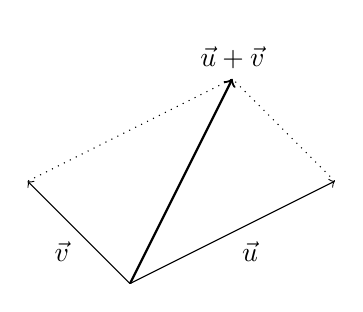
\begin{tikzpicture}[scale=1.3]
	\clip (-1,0) rectangle (2,2.5);

	% \vec u
	\draw[thin] [->] (0,0) -- (2,1);
	\draw (1,0.5) node[anchor=north west] {$\vec u$};

	% \vec v
	\draw[thin] [->] (0,0) -- (-1,1);
	\draw (-0.5,0.5) node[anchor=north east] {$\vec v$};

	% \vec u + \vec v
	\draw[thick] [->] (0,0) -- (1,2);
	\draw (1,2) node[anchor=south] {$\vec u + \vec v$};

	% Help lines
	\draw[dotted] [-] (2,1) -- (1,2) -- (-1,1);

\end{tikzpicture}}

			\item
			Pela definição da subtração de vetores, isto é, $\vec u - \vec v \mycoloneqq \vec u + (-\vec u)$:
			\inlinebox{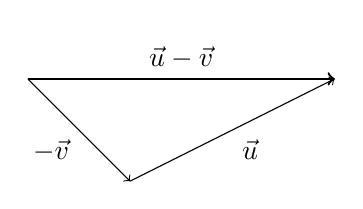
\begin{tikzpicture}[scale=1.3]
	\clip (-1,0) rectangle (2,1.5);

	% \vec u
	\draw[thin] [->] (0,0) -- (2,1);
	\draw (1,0.5) node[anchor=north west] {$\vec u$};

	% \vec -v
	\draw[thin] [<-] (0,0) -- (-1,1);
	\draw (-0.5,0.5) node[anchor=north east] {$-\vec v$};

	% \vec u + \vec v
	\draw[thick] [->] (-1,1) -- (2,1);
	\draw (0.5,1) node[anchor=south] {$\vec u - \vec v$};

\end{tikzpicture}}

			\item
			$\frac{3}{2}\vec u \parallel \vec u$ e seu comprimento é $3/2$ vezes o de $\vec u$:
			\inlinebox{\begin{tikzpicture}[scale=1.3]
	\clip (-1,0) rectangle (3,2);

	% 3/2 \vec u
	\draw[thick] [->] (0,0) -- (3,3/2);
	\draw (9/4,9/8) node[anchor=north west] {$\frac{3}{2}\vec u$};

	% \vec u
	\draw[thin] [->] (0,0) -- (2,1);
	\draw (1,0.5) node[anchor=north west] {$\vec u$};

	% \vec v
	\draw[thin] [->] (0,0) -- (-1,1);
	\draw (-0.5,0.5) node[anchor=north east] {$\vec v$};

\end{tikzpicture}}
		\end{enumerate}
	\end{solution}
\end{question}
